\subsection{O3: does pre-processing strengthen the blur signature?}
\label{sec:preproc}
Every candidate was inserted in front of the same estimator and run on the same test trials as
Section~\ref{sec:sweep} (8{,}960 trials per variant). Figure~\ref{fig:preproc} and
Table~\ref{tab:preproc} show the result.

\begin{figure}[h]
\centering
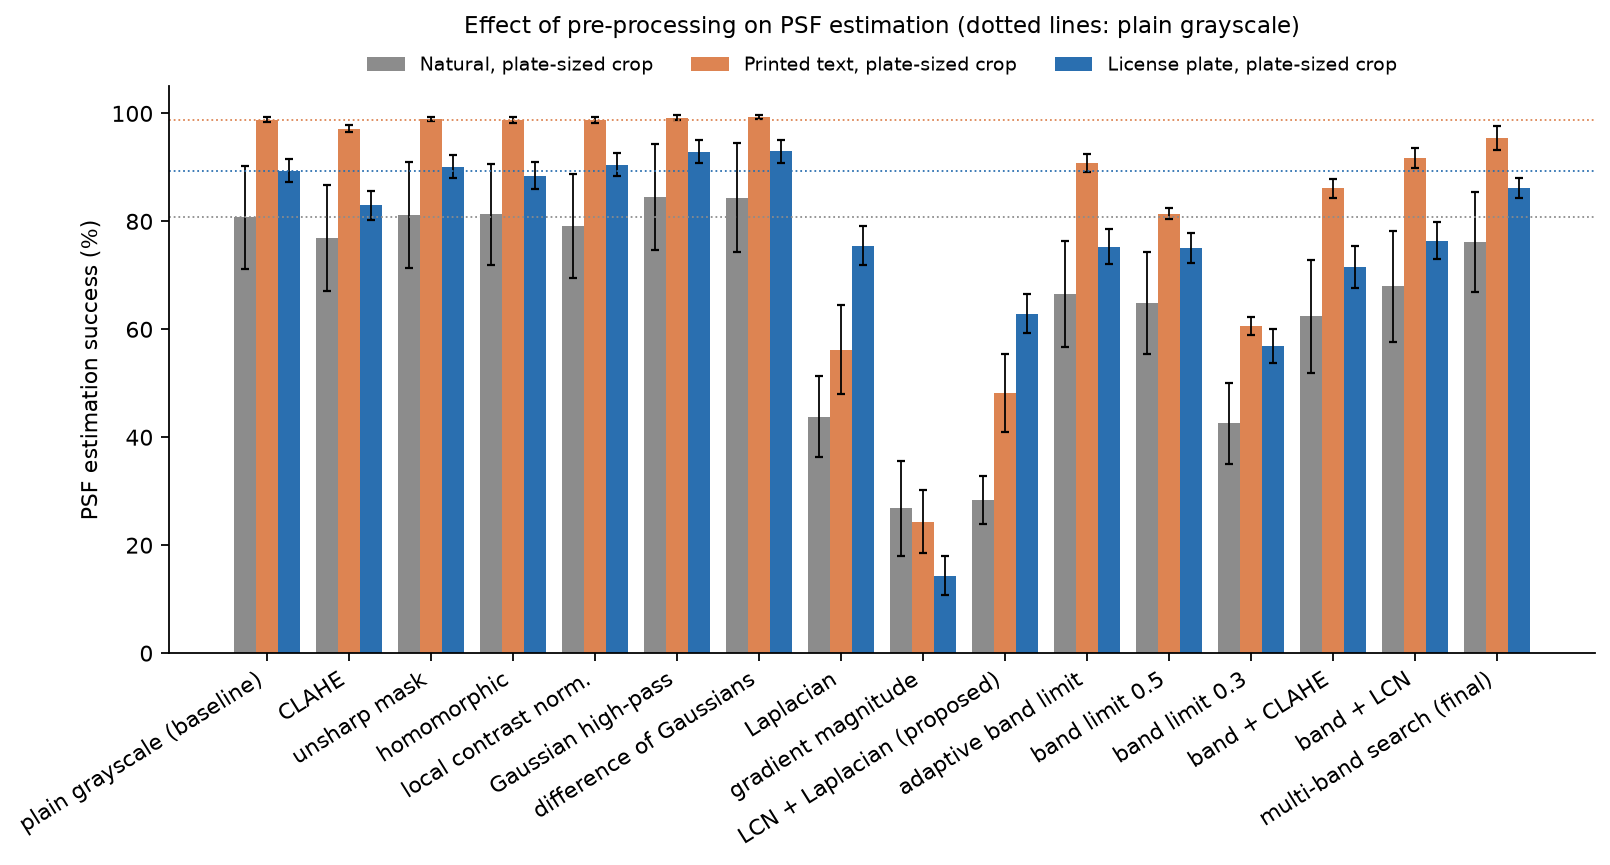
\includegraphics[width=\textwidth]{03_preprocess_success.png}
\caption{Estimation success per pre-processing variant (test split; dotted lines: plain grayscale).}
\label{fig:preproc}
\end{figure}

\begin{table}[h]
\centering\small
\begin{tabular}{lcccc|cc}
\toprule
variant & natural & text & plate & mean & plate, $L{=}5$ & plate, $\sigma{=}0.04$ \\
\midrule
plain grayscale (baseline) & 80.7 & 98.9 & 89.4 & 89.7 & 58 & 76 \\
CLAHE & 77.0 & 97.2 & 83.0 & 85.7 & 33 & 70 \\
unsharp mask & 81.2 & 99.0 & 90.1 & 90.1 & 61 & 76 \\
local contrast normalisation & 79.2 & 98.8 & 90.5 & 89.5 & 63 & 78 \\
Gaussian high-pass & \textbf{84.5} & 99.2 & \textbf{92.9} & \textbf{92.2} & \textbf{73} & \textbf{82} \\
difference of Gaussians & 84.4 & \textbf{99.3} & \textbf{92.9} & \textbf{92.2} & \textbf{73} & \textbf{82} \\
Laplacian & 43.8 & 56.2 & 75.5 & 58.5 & 62 & 22 \\
gradient magnitude & 26.8 & 24.4 & 14.3 & 21.8 & 20 & 9 \\
LCN + Laplacian (proposed) & 28.4 & 48.2 & 62.9 & 46.5 & 58 & 3 \\
adaptive band limit & 66.6 & 90.7 & 75.3 & 77.5 & 17 & 62 \\
band limit 0.3 & 42.6 & 60.6 & 57.0 & 53.4 & 0 & 54 \\
multi-band search (final) & 76.2 & 95.5 & 86.1 & 85.9 & 44 & 73 \\
\bottomrule
\end{tabular}
\caption{Estimation success (\%) on the synthetic test split. Homomorphic filtering and the band
limits combined with CLAHE/LCN are in \texttt{results/csv/03\_summary.csv}.}
\label{tab:preproc}
\end{table}

\paragraph{Findings.} The proposed stage --- local contrast normalisation followed by Laplacian edge
enhancement --- \emph{lowers} success from 89.7\% to 46.5\% and collapses under noise (3\% on
plates at $\sigma=0.04$). Strong derivative operators (Laplacian, gradient magnitude) behave the
same way: they multiply the spectrum by $|\omega|^2$ or worse, so the high-frequency noise floor
swamps the nulls and the operator's own structure adds spurious dips. Contrast normalisation alone
(CLAHE, LCN, homomorphic) is neutral to slightly harmful.

The one family that helps on synthetic data is the \emph{mild} band-pass: a Gaussian high-pass or
difference of Gaussians gains $+2.5$ points overall and $+15$ points on plates at $L=5$, the
failure pocket of Section~\ref{sec:sweep}. It flattens the strong low-frequency fall-off of the
spectrum without amplifying the noise band. These two operators were not part of the
development comparison on real plates (Section~\ref{sec:design}), so --- to avoid choosing on
test data --- they were not adopted; testing them on real plates is the most direct follow-up.

The final multi-band search costs 3.8 points here, all of it on short blurs ($L=5$: 44\% vs.\
58\% on plates), where the first null lies outside the lower bands and the full-band candidate
does not always win the directionality comparison. It was chosen for real plates, where it is
decisive (Section~\ref{sec:real}); on synthetic data, where noise is white and there is no
compression or resampling, the full spectrum carries real information up to Nyquist.
